%%%%%%%%%%%%%%% Pacotes utilizados
\documentclass[a4paper, 12pt]{article}
\usepackage[T1]{fontenc}
\usepackage[brazil]{babel}
\usepackage[utf8]{inputenc}
\usepackage{verbatim}
\usepackage[normalem]{ulem} %para 
\usepackage{indentfirst}
\usepackage{setspace}
\usepackage{float}
\usepackage{fancyhdr}
\usepackage{titlesec}
\usepackage{capt-of}
\usepackage{setspace}
\usepackage{graphicx}
\usepackage{booktabs}

%%%%%%%%%%%%%%% Configurações
\setlength{\textwidth}{16cm}
\setlength{\textheight}{23cm}
\setlength{\evensidemargin}{-1cm} 
\setlength{\oddsidemargin}{0.5cm}
\setlength{\topmargin}{0cm}
\pagestyle{fancy}
\fancyhf{}
\lhead{\textbf{Nome:} Jhonatan Guilherme de Oliveira Cunha}
\rhead{\textbf{RA:} 2135590}
\cfoot{\thepage}
\hoffset= -0.4cm
\voffset=-0.9cm

\setstretch{1.5}

\titleformat{\chapter}{\normalfont\huge}{\textbf{\thechapter.}}{20pt}{\huge\bf}


%%%%%%%%%%%%% Início do documento
\begin{document}
	\hspace{2cm}

	\begin{large}
		\begin{center}
			\textbf{UNIVERSIDADE TECNOLÓGICA FEDERAL DO PARANÁ}\newline
			\textbf{CAMPUS CAMPO MOURÃO}
		\end{center}
	\end{large}
	
	\vspace{0.5cm}
	
	\begin{center}
		\textbf{Diagrama e descrição textual dos casos de uso - Sistema Clínica Veterinária}
	\end{center}


	\section{Diagrama caso de uso}
	
	Conforme solicitado na descrição da atividade, deveríamos implementar a modelagem do diagrama de caso de uso da \textbf{UML}. Veja na Figura \ref{fig:DiagramaCasoUso} o resultado da tarefa mencionada.
	
	\begin{figure}[H]
		\centering
		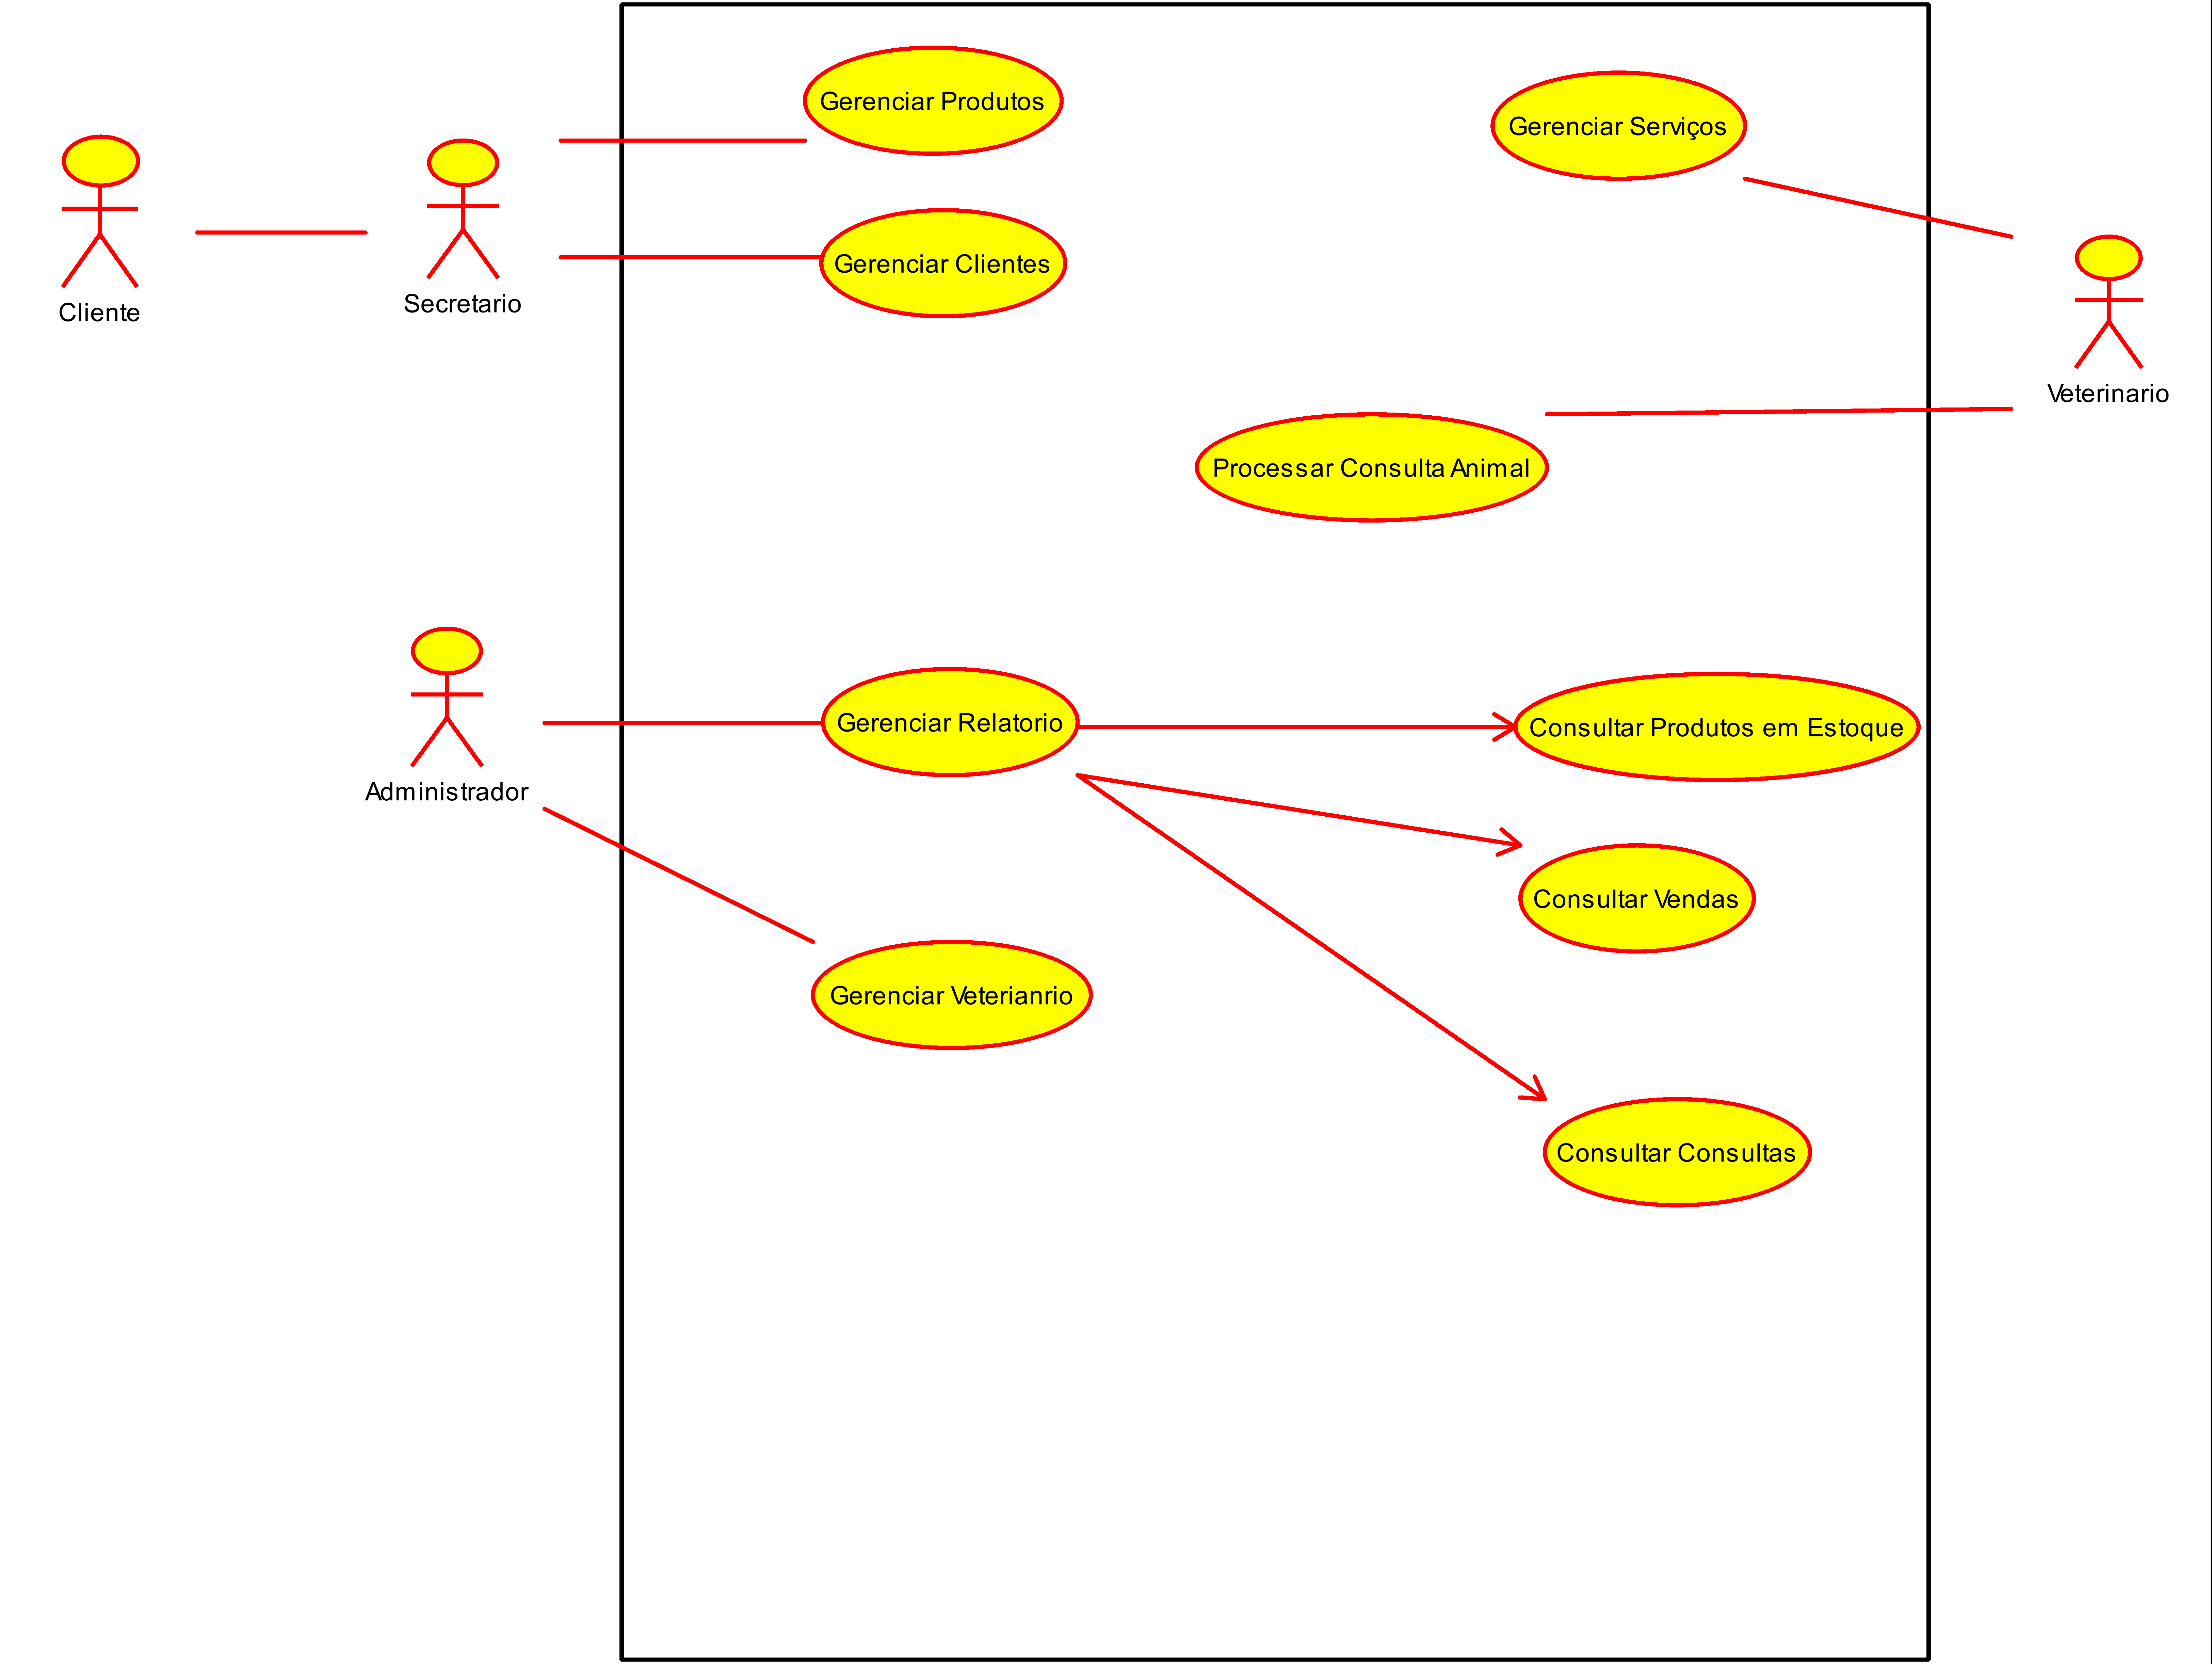
\includegraphics[width=1\textwidth]{caso.png}
		\label{fig:DiagramaCasoUso}
		\caption{Diagrama \textbf{UML} de caso de uso.}		
	\end{figure}
	
	Analisando o diagrama acima, na próxima seção descreveremos em textos todos os casos de uso acima, balanceando entre resumido, completo abstrato e concreto.
	
	\section{Descrições Textuais}
	
	\begin{table}[H]
		
		\centering
		\begin{tabular}{p{0.2\linewidth}  p{0.8\linewidth}}
			\toprule
			
			\textbf{Caso de Uso:} & Gerenciar Produtos\\ \midrule
			\textbf{Visão Geral:} & O secretario tem o poder de gerenciar todas as informações de produtos disponíveis no sistema, realizando ações básicas como: alterar, remover e inserir produtos. Além disso, terá a permissão de controlar as categorias de cada produto. \\ 
	
			\bottomrule
		\end{tabular}
	\caption{ {\small Formato Resumido.}}
	\end{table}

	\vspace{2cm}

	\begin{table}[H]
		\centering
		\begin{tabular}{p{0.3\linewidth}  p{0.7\linewidth}}
			\toprule
			
			\textbf{Caso de Uso:} & Processar Consulta Animal\\ \midrule
			\textbf{Ator Principal:} & Veterinário \\ \midrule
			\textbf{Interessados e Interesses:} & 
				\begin{itemize}
					\item Veterinário: deseja informar ao sistemas todas as informações necessárias para um consulta aplica em algum animal da clínica veterinária.

				\end{itemize} \\ \midrule
			\textbf{Pré-Condições} & O veterinário está autenticado e identificado. \\ \midrule
			\textbf{Pós-Condições:} & O sistema armazenará qual veterinário realizou a consulta. \\ \midrule
			\textbf{Cenário de Sucesso Principal:} & 
			\begin{enumerate}
				\item O veterinário abre o sistema.
				\item O veterinário entra no modulo de consulta do sistema.
				\item O veterinário informa todos os dados da consulta que o mesmo quer processar.
				\item A consulta é processada com sucesso.
			\end{enumerate} \\ \midrule
			
			\textbf{Fluxo Alternativo 1:} & A qualquer momento o veterinário pode cancelar o processamento durante o processo. \\ \midrule
			\textbf{Fluxo Alternativo 2:} & 3. O sistema informa ao veterinário que as informações passadas são inválidas. Solicitando novamente ao veterinário os dados corretos. \\ \midrule
			\textbf{Fluxo Alternativo 3:} & 4. O sistema por algum motivo não consegue registrar no banco de dados a consulta. Guardar os dados para tentar realizar novamente a requisição mais tarde. \\ \midrule
			\textbf{Fluxo Alternativo 4:} & - \\ 
			
			\bottomrule
		\end{tabular}
		\caption{ {\small Formato Abstrato.}}
	\end{table}


	\begin{table}[H]
		\centering
		\begin{tabular}{p{0.3\linewidth}  p{0.65\linewidth}}
			\toprule
			
			\textbf{Caso de Uso:} & -\\ \midrule
			$\dots$ &  \\ \midrule
			$\dots$ &  \\ \midrule
			$\dots$  \\ \midrule
			$\dots$&  \\ \midrule
			\textbf{Cenário de Sucesso Principal:} & -  \\ 
			
			\bottomrule
		\end{tabular}
		\caption{ {\small Formato Concreto.}}
	\end{table}
	
	
\end{document}
